\section{Background}\label{sec:background}
% General introduction
The exponential tendency for data demand to the \textit{zettabyte} era, predicted by major network providers \cite{cisco2016forecast,kremling2015presentation,belllabs2016report,ericsson2015report}, is present and evident. The use of cellular networks for data consumption has become a widespread topic to the general audience. The reason has been the flourishement of online applications services from the last two decades such as:  Whatsapp, Viber (voice and messaging), Facebook, Twitter, Snapchat, Instagram, Google+ (social networking), YouTube, Netflix, SoundCloud, Spotify (video or audio streaming), Google Drive, Dropbox and OneDrive (data storage). Also, these applications have been developed not only for a \ac{PC} but also mobile smartphones, tablets and phablets that support either the Android, iOS or Windows Mobile \ac{OS}. Further, content delivery networks will be carrying two-thirds of the Internet traffic by the end of 2016 \cite{cisco2016forecast}. Hence, it is expected that the data growth will continue within this market. From all these services, streaming applications that are based in multicast scenarios where a transmitter needs to serve tens, hundreds or even thousands of receivers are becoming more frequent in mobile networks such as \ac{LTE-A} or \ac{WLAN} networks such as \ac{WiFi}. These types of scenarios pose tight requirements in terms of data throughput and delay to ensure a satisfactoring \ac{QoE}.

For the network operator, techniques that can offload the service infrastructure to cope with such data load are needed in order to satisfy the increasing demand. Further, due to network capacity constraints, the end-user might not be connected to a \ac{BS} in a cellular fashion. Instead, the connectivity might be provided by other users either within the cellular spectrum or through a \ac{WLAN}. The deployment of mobile devices without cellular coverage but in a local network can potentially be decentralized. This type of deployment will require the communicating devices to (i) employ multihop communications to ensure connectivity, (ii) use control access mechanisms to avoid interference in the local network. From the devices perspective, energy consumption due to data transmissions has become a limiting factor in terms of battery life. The reason is that mobile devices perform much more internal tasks than older devices from ten years ago. Therefore, mobile network designers need to consider mechanisms and techniques that aim for high throughput and low energy consumption both at the station and the end user devices and that are able to provide data offloading from current network infrastructures.

\subsection{Cooperative Wireless Networks}
% Cooperation
The concept of cooperation in wireless networks has been investigated before \cite{fitzek2006cooperation,fitzek2007cognitive,heide2012green,fitzek2013implementation,fitzek2013mobile}. The main goal is to diminish the amount of communications resources (data rate, energy or even storage and computational power) to convey an information of common interest from a transmitter to a set of interconnected receivers in a multicast fashion. Devices connected in this way form a \textit{mobile cloud} \cite{fitzek2013mobile}. In Fig.~\ref{fig:cooperation}, it can be observed a comparison example of no cooperation and cooperation in a multicast wireless network.

\begin{figure}[ht!]
  \centering 
  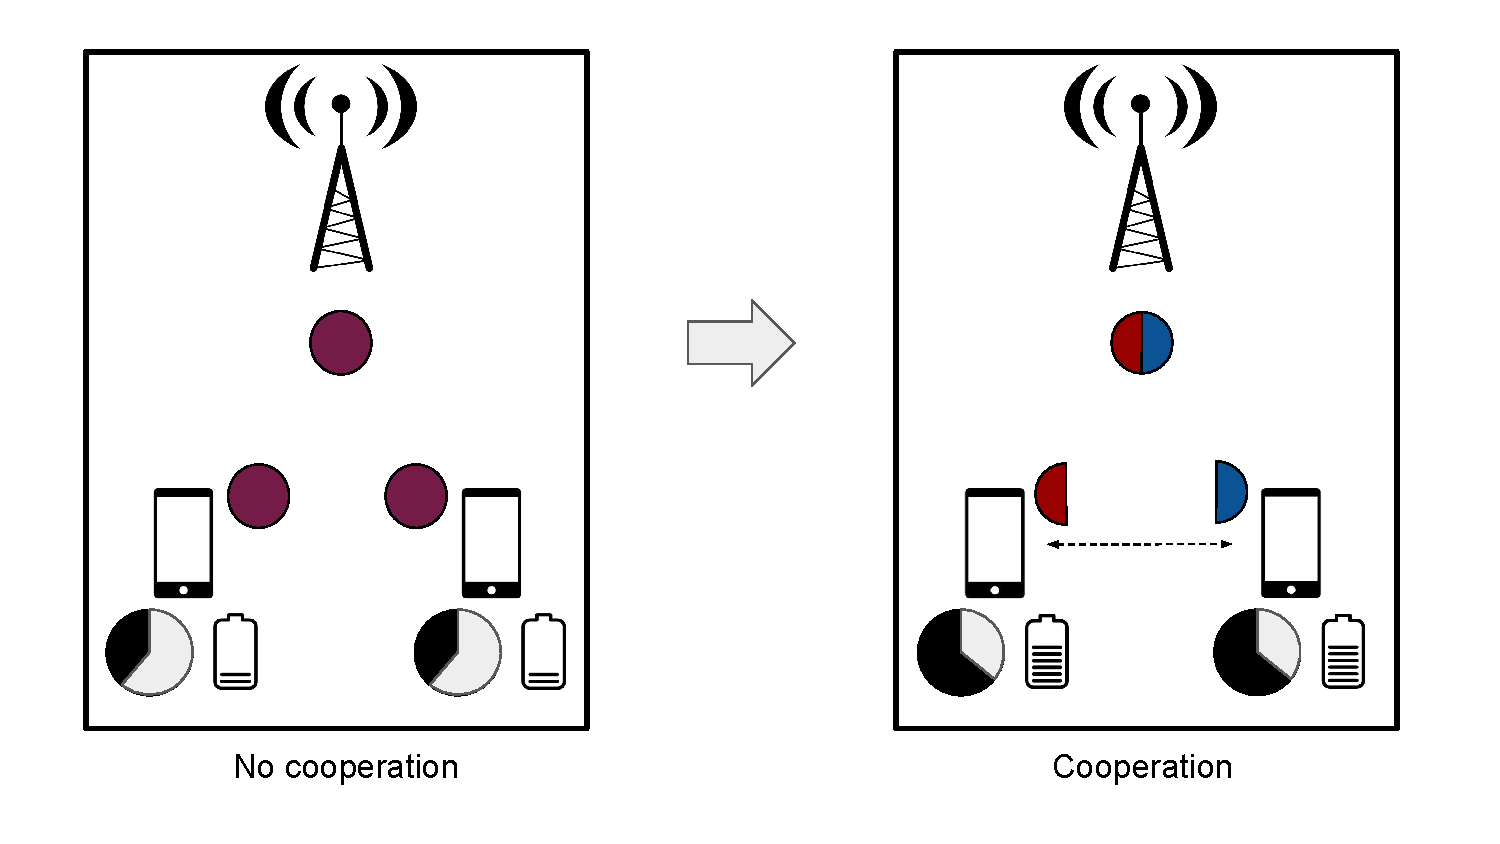
\includegraphics[width=\textwidth]{introduction/figures/cooperation.pdf}
  \caption{Cooperation in Wireless Networks.}
\label{fig:cooperation}
\end{figure} 

Without cooperation, a purple content is sent to two mobile devices in a broadcast fashion. This incurs in posible a large downloading time to ensure both devices are satisfied reducing the throughput and increasing the energy consumption.  When cooperation is considered, the content now is split into smaller blue and red pieces where each of them is sent rapidly to each device. Then, the devices exploit short-range communications (dashed line) by exchanging their missing pieces. The key underlying idea is for the devices share their missing information through a faster, short-distance and reliable link which increases the total throughput and reduces the overal energy consumption. From an operator perspective, the information \textit{as a whole} is quickly disseminated into the receivers helping the \ac{BS} to offload data. At the end, the goal of making the cluster share resources is achieved. In this way, mobile clouds allow to improve the overall network performance and user experience.

\subsection{Device to Device and Erasure Correcting Codes}
\label{sec:d2d_erasure_codes}
One of the key aspects to achieve the gains proposed by the cooperative approach is the short-range technology to be considered and its parameters to guarantee a fast and reliable link. Besides \ac{WLAN} technologies such as Bluetooth or \ac{WiFi}, there has been a large interest in \ac{D2D} communications \cite{lin2013comprehensive,asadi2014survey,feng2014device,tehrani2014device}. Device discovery, communication resource allocation and coordination for these type of communications are principally considered to be handled by the cellular. This permits the devices to share data without going through the cellular network which keeps the idea of data offloading. Furthermore, \ac{D2D} based \ac{ProSe} have been included in \cite{3gpp2012prose} to use them in \ac{LTE-A} networks for an improved \ac{QoE}.

Another aspect that is relevant for cooperation gains in multicast scenarios is channel coding. Due to the dynamics of the wireless medium, propagation conditions, noise and interference may degradate the received \ac{SINR} thus making reception unfeasible for some period of time. In the case of packet networks this leads to \textit{erasure} channels where packets are either correctly received or lost. Therefore, to protect against packet erasures, some redundancy is added through channel coding with a \ac{FEC} technique also called an erasure correcting code. These techniques are relevant to make multicast applications reliable since feedback control through \ac{ACK} packets is not possible for a large number of devices.

Different erasure correcting codes might be used for reliable multicast applications. In the literature, we can find linear block codes such as \ac{RS} \cite{reed1960polynomial} or \ac{LDPC} \cite{gallager1962low}. More recently, \ac{LT} codes \cite{luby2002lt} and Raptor codes \cite{shokrollahi2006raptor} are codes that are more adaptable to the channel conditions that block codes. These latter type of codes are characterized by being: (i) Able to generate a very large number of coded symbols, i.e rateless, (ii) close-to-optimal, i.e requiring a slightly higher amount of encoded symbols than the original set to decode and (iii) able to decode with a subset of coded symbols as long as there are no inter-dependencies in it.

Although these coding techniques are useful for multicast networks, they pose two major restrictions to apply them with the cooperative approach. First, this type of coding is made on a \textit{link} basis, meaning that for each hop encoding and decoding needs to take place. The required code processing for each hop brings delays and energy consumption due to computational aspects. Second, as a consequence of the previous, these codes are not composable in principle. This implies that there are no known forms to create new coded packets from packets that have been coded previously without decoding in the case of rateless codes. Because of these limitations state of the art rateless codes are not ideal erasure correcting codes for cooperative wireless networks with \ac{D2D} due to the inherent processing in multihop.

\subsection{Network Coding}
\label{sec:nc_rlnc}
% Network Coding, inter-session (XOR) and intra-session (RLNC)
Introduced by Alshwede et al. \cite{ahlswede2000network}, \ac{NC} appeared as an effective technology to remove the limitations presented previously. In this work, the authors presented a new paradigm shift for conveying information in communication networks. Instead of treating the packets as atomic unmodifiable units at the intermediate node in an example network known as the \textit{butterfly network}, they are regarded as algebraic elements in a \ac{GF} that can be operated on to create new coded packets. In \cite{ahlswede2000network}, the authors considered the binary field to perform the algebraic operations. This type of coding bevcame known later as inter-session network coding since packets from two sessions where mixed in the coding process. Due to the binary field nature, it also became known as XOR coding since this operation is congruent with the modulo-2 addition.

Besides inter-session network coding, intra-session network coding also known as \ac{RLNC} \cite{ho2006random} was introduced by Ho et al. Here, coded packets are algebraic linear combinations of original set of packets from a single data flow. This permits to remove the limitation of sending \textit{particular} packets by now sending coded packets as linear equations of the originals. This new type of coding across the network is proven to achieve the multicast capacity from a flow perspective with very high probability \cite{koetter2003algebraic,ho2006random}. Later, this key idea let the research community know for the first time that it was possible to code on a \textit{network} basis and not only on a link basis as conventional \ac{FEC} technologies do. In this way, instead of typically encoding and decoding on a hop basis, relaying nodes can recode packets to reduce delay and still take advantage of the data representation for the next hop. In this sense, \ac{RLNC} appears as the only coding technique that overcomes the restrictions mentioned in Section~\ref{sec:d2d_erasure_codes}.

\textbf{RLNC DESCRIPTION AND TABLE SHOWING THE TRADEOFF BETWEEN HIGH AND LOW FIELDS}

\subsection{Thesis Objectives}
Based in the previous background, this thesis considers to push the state of the art by using multicast \ac{D2D} mobile clouds in cooperative wireless networks with \ac{RLNC} since current techniques focuses mostly in \ac{D2D} communications based in unicast pairs with either \ac{RLNC} or non-composable rateless codes. The objectives of this thesis are to:

\begin{enumerate}

\item Define the regions and conditions in terms of network and code parameters parameters where cooperation with \ac{RLNC} provides a better performance than broadcast with \ac{RLNC} in terms of data throughput and energy consumption at the mobile devices.

\item Propose and study code constructions that permit to avoid the \ac{RLNC} tradeoff from Section~\ref{sec:nc_rlnc} to achieve minimum total overhead. In this sense, the objective is to find codes that permit to retain the low coding coefficients overhead from a low field size, but also the low number of transmissions overhead from high fields. 

\item Study the dominating regimes and ideal cloud sizes to observe if there exists ideal values for high system throughput and low energy consumption.

\item Study the effect of transmission policies under a \ac{WLAN} scenario. In this case, medium access mechanisms to avoid interference should be considered.
\end{enumerate}

\begin{figure}[ht!]
  \centering 
  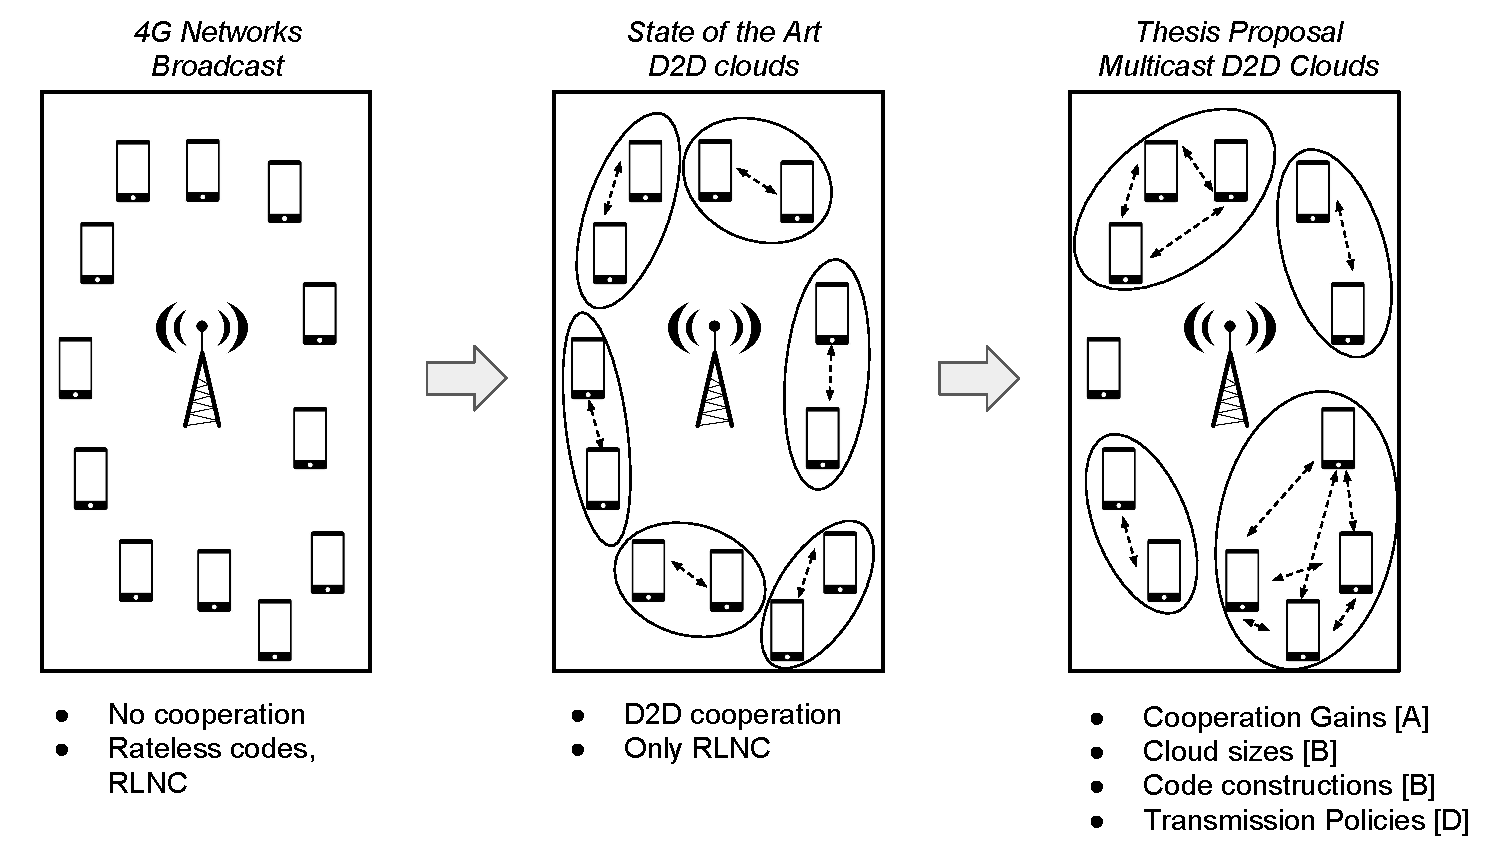
\includegraphics[width=\textwidth]{introduction/figures/thesis-diagrams.pdf}
  \caption{State of the Art and Thesis Proposal.}
\label{fig:proposal}
\end{figure}

From Fig.~\ref{fig:proposal}, the study for objective 1 was addressed in paper {[\ref{paper:paperA}]}. Objectives 2 and 3 were reviewed in paper {[\ref{paper:paperB}]}. Finally, objective 4 was addressed in paper {[\ref{paper:paperD}]} with a software tool implemented in paper {[\ref{paper:paperC}]} that uses Kodo and the open-source ns-3 simulator \cite{ns3link}.

%In principle, adding more users to the cloud enhances the realibility of it and minimizes the transmissions from the \ac{BS}. Still, this might increment the transmissions inside the clouds since . 
